\section{Photodiode}

Solid state detectors like the photodiode are based on the properties of semiconductors. These types of detectors have marked advantages over other types of detectors, they can be kept smaller than gas-filled detectors due to their density and also have better energy resolution than the scintillator counters \cite[Chap 11.]{knollRadiationDetectionMeasurement2010}. In this section, we will discuss the basic concepts of semiconductors and how they can be used as detectors.

\subsection{Semiconductors}
\subsubsection{Band Structure and Charge Carriers}

In crystalline solid materials, the periodic lattice structures restrict electron energies to distinct allowed bands that are separated by forbidden energies as shown in the diagram \cref{fig:band_structure}. The lower of these energy regions, known as the valence band, contains outer-shell electrons that are placed in a specific position inside the lattice via interatomic bonds. Conversely, the higher-lying conduction band represents free electrons capable of migrating through the crystal lattice and this electrons allow  electrical conductivity to be present. The magnitude of the forbidden energy gap or bandgap between these two bands dictates whether a material functions as an insulator or a semiconductor. 

In the absence of thermal excitation, both insulators and semiconductors maintain a completely filled valence band and a completely empty conduction band, resulting in no electrical conductivity under these baseline conditions. In contrast, metals feature not entirely filled highest energy band, permitting electrons to easily migrate within the crystal lattice with minimal incremental energy and thus ensuring high electrical conductivity across the material. For insulators and semiconductors, however, electrons must first cross the intervening bandgap to reach the conduction band, causing their baseline electrical conductivity to be many orders of magnitude lower \cite[Chap 11.]{knollRadiationDetectionMeasurement2010}.

\begin{figure}[htbp]
    \centering
    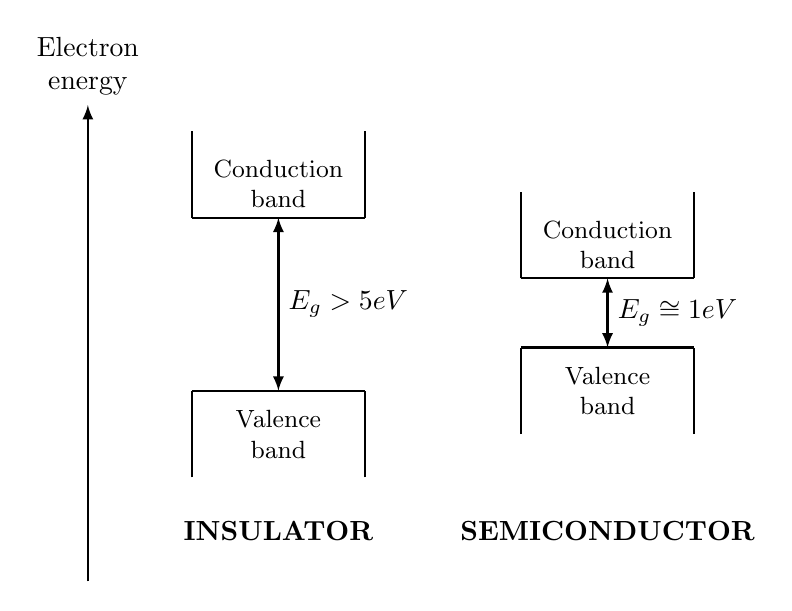
\begin{tikzpicture}[scale=1.1, >=latex]
        % Eje de energía vertical
        \draw[->, thick] (0,0) -- (0,5.5) node[above, align=center] {Electron\\energy};

        % --- AISLANTE (INSULATOR) ---
        \begin{scope}[shift={(1.2,0)}]
            % Banda de conducción
            \draw[thick] (0,4.2) -- (2.0,4.2);
            \node[above, align=center, font=\small] at (1.0,4.2) {Conduction\\band};
            \draw[thick] (0,4.2) -- (0,5.2);
            \draw[thick] (2.0,4.2) -- (2.0,5.2);

            % Flecha de banda prohibida (Eg > 5 eV)
            \draw[<->, thick] (1.0,2.2) -- node[right, align=left] {$E_g > 5\text{ eV}$} (1.0,4.2);

            % Banda de valencia
            \draw[thick] (0,2.2) -- (2.0,2.2);
            \draw[thick] (0,1.2) -- (0,2.2);
            \draw[thick] (2.0,1.2) -- (2.0,2.2);
            \node[align=center, font=\small] at (1.0, 1.7) {Valence\\band};

            % Etiqueta inferior
            \node[below, font=\bfseries] at (1.0, 0.8) {INSULATOR};
        \end{scope}

        % --- SEMICONDUCTOR ---
        \begin{scope}[shift={(5.0,0)}]
            % Banda de conducción
            \draw[thick] (0,3.5) -- (2.0,3.5);
            \node[above, align=center, font=\small] at (1.0,3.5) {Conduction\\band};
            \draw[thick] (0,3.5) -- (0,4.5);
            \draw[thick] (2.0,3.5) -- (2.0,4.5);

            % Flecha de banda prohibida (Eg ≈ 1 eV)
            \draw[<->, thick] (1.0,2.7) -- node[right, align=left] {$E_g \cong 1\text{ eV}$} (1.0,3.5);

            % Banda de valencia
            \draw[thick] (0,2.7) -- (2.0,2.7);
            \draw[thick] (0,1.7) -- (0,2.7);
            \draw[thick] (2.0,1.7) -- (2.0,2.7);
            \node[align=center, font=\small] at (1.0, 2.2) {Valence\\band};

            % Etiqueta inferior
            \node[below, font=\bfseries] at (1.0, 0.8) {SEMICONDUCTOR};
        \end{scope}

    \end{tikzpicture}
    \caption{Band structure for electron energies in insulators and semiconductors \cite[Chap 11.]{knollRadiationDetectionMeasurement2010}.}
    \label{fig:band_structure}
\end{figure}

At any temperature greater than zero the thermal energy introduced into the electrons within the lattice allows them to gain sufficient energy to cross the bandgap into the conduction band, leaving behind a vacancy known as a hole. This combination forms an electron-hole pair. Under the influence of an applied electric field, conduction electrons migrate toward positive potentials while positive holes move in the opposite direction, with the motion of both charge carriers contributing directly to the material's observed electrical conductivity. 

\begin{equation}
    p(T) = C T^{3/2} \exp\left(-\frac{E_g}{2kT}\right)
    \label{eq:thermal_generation}
\end{equation}

where:
\begin{itemize}
    \item $T =$ absolute temperature
    \item $E_g =$ bandgap energy
    \item $k =$ Boltzmann constant
    \item $C =$ proportionality constant characteristic of the material
\end{itemize}

The probability per unit time for thermal electron-hole pair generation is given by \cref{eq:thermal_generation} in \cite[p. 367]{knollRadiationDetectionMeasurement2010}. This generation of electron-hole pairs is heavily dependent on the ratio of the bandgap energy to the absolute temperature of the material. Consequently, materials with bigger bandgaps experience minimal thermal excitation that could create conductivity and thus act as insulators, while materials with smaller bandgaps yield sufficient conductivity to be classified as semiconductors. When there is no electric field pulling them apart, the electrons and holes created by heat eventually find each other and recombine canceling each other out. They constantly form and recombine until they reach a stable balance, this balance depends heavily on heat. If the material is cooled down, there is less thermal energy available, causing the number of active electron-hole pairs to drop drastically.


\subsubsection{Effect of Impurities on Semiconductors}

An ideal semiconductor without any traces of other elements or impurities is called an intrinsic semiconductor. The conductivity is then only determined by the electrons and holes generated by thermal excitation. However, in practice it is almost impossible to have a pure semiconductor, and the presence of impurities can significantly alter the electrical properties of the material. The process of intentionally adding impurities to a semiconductor is known as doping, and it can create two types of extrinsic semiconductors: n-type and p-type.

\begin{figure}[htbp]
    \centering
    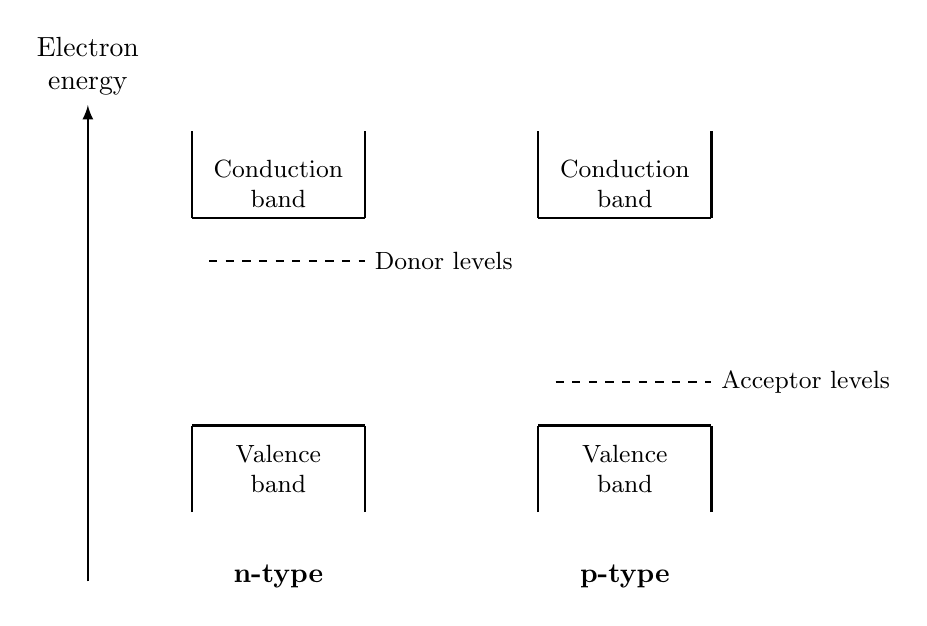
\begin{tikzpicture}[scale=1.1, >=latex]
        % Eje de energía vertical compartido
        \draw[->, thick] (0,0) -- (0,5.5) node[above, align=center] {Electron\\energy};

        % ==========================================
        % 1. N-TYPE SEMICONDUCTOR (Donor levels)
        % ==========================================
        \begin{scope}[shift={(1.2,0)}]
            % Banda de conducción
            \draw[thick] (0,4.2) -- (2.0,4.2);
            \node[above, align=center, font=\small] at (1.0,4.2) {Conduction\\band};
            \draw[thick] (0,4.2) -- (0,5.2);
            \draw[thick] (2.0,4.2) -- (2.0,5.2);

            % Niveles donantes (línea discontinua)
            \draw[thick, dashed] (0.2, 3.7) -- (2.0, 3.7);
            \node[right, font=\small] at (2.0, 3.7) {Donor levels};

            % Banda de valencia
            \draw[thick] (0,1.8) -- (2.0,1.8);
            \draw[thick] (0,0.8) -- (0,1.8);
            \draw[thick] (2.0,0.8) -- (2.0,1.8);
            \node[align=center, font=\small] at (1.0, 1.3) {Valence\\band};

            % Etiqueta inferior
            \node[below, font=\bfseries] at (1.0, 0.3) {n-type};
        \end{scope}

        % ==========================================
        % 2. P-TYPE SEMICONDUCTOR (Acceptor levels)
        % ==========================================
        \begin{scope}[shift={(5.2,0)}]
            % Banda de conducción
            \draw[thick] (0,4.2) -- (2.0,4.2);
            \node[above, align=center, font=\small] at (1.0,4.2) {Conduction\\band};
            \draw[thick] (0,4.2) -- (0,5.2);
            \draw[thick] (2.0,4.2) -- (2.0,5.2);

            % Banda de valencia
            \draw[thick] (0,1.8) -- (2.0,1.8);
            \draw[thick] (0,0.8) -- (0,1.8);
            \draw[thick] (2.0,0.8) -- (2.0,1.8);
            \node[align=center, font=\small] at (1.0, 1.3) {Valence\\band};

            % Niveles aceptores (línea discontinua y etiqueta a la derecha)
            \draw[thick, dashed] (0.2, 2.3) -- (2.0, 2.3);
            \node[right, font=\small] at (2.0, 2.3) {Acceptor levels};

            % Etiqueta inferior
            \node[below, font=\bfseries] at (1.0, 0.3) {p-type};
        \end{scope}

    \end{tikzpicture}
    \caption{Band structures for n-type (donor levels near the conduction band) and p-type (acceptor levels near the valence band) doped semiconductors \cite[Chap 11.]{knollRadiationDetectionMeasurement2010}.}
    \label{fig:band_structure_doped}
\end{figure}

\begin{itemize}
  \item \textbf{N-type Semiconductors:} When an impurity atom with more valence electrons than silicon is introduced into a silicon crystal lattice as dopants, they substitute for regular silicon atoms and provide an extra valence electron beyond what is needed for covalent bonding. These loosely bound electrons occupy discrete donor energy levels located near the top of the forbidden bandgap as shown in \cref{fig:band_structure_doped}, where minimal thermal energy is sufficient to ionize them into the conduction band. Consequently, the concentration of conduction electrons becomes overwhelmingly dominated by these donor contributions rather than intrinsic thermal generation. This massive increase in conduction electrons accelerates recombination rates, shifting the equilibrium to sharply reduce the concentration of holes. As a result, these kinds of semiconductors achieve significantly higher electrical conductivity than pure intrinsic materials, with electrons functioning as the majority carriers and holes as the minority carriers. Despite this imbalance in mobile charge carriers, overall electrical neutrality is perfectly maintained by the fixed, positively charged ionized donor sites permanently locked within the crystal lattice.
  \item \textbf{P-type Semiconductors:} When an impurity atom with less valence electrons than silicon is introduced into a silicon crystal lattice as a dopant, it substitutes for a regular silicon atom and provides one fewer valence electron than is needed for covalent bonding, thereby leaving an unsaturated bond or hole. These vacancies occupy discrete acceptor energy levels located near the bottom of the forbidden bandgap as shown in \cref{fig:band_structure_doped}, where minimal thermal energy allows electrons from normal covalent bonds to fill them, leaving mobile holes behind in the valence band. Consequently, the concentration of holes becomes overwhelmingly dominated by these acceptor contributions rather than intrinsic thermal generation. This massive increase in holes accelerates recombination rates with conduction electrons, shifting the equilibrium to sharply reduce the concentration of conduction electrons. As a result, these kinds of semiconductors achieve significantly higher electrical conductivity than pure intrinsic materials, with holes functioning as the majority carriers and electrons as the minority carriers. Despite this imbalance in mobile charge carriers, overall electrical neutrality is perfectly maintained by the fixed, negatively charged ionized acceptor sites permanently locked within the crystal lattice.
\end{itemize}

\subsection{Semiconductors as Detectors}

Semiconductor sensors operate by capturing incident photons and converting them into measurable electrical charges through the internal photoelectric effect. This effect relies on the absorption of photons with energies ($h\nu$) exceeding the semiconductor's bandgap, which excites electrons from the valence band to the conduction band, leaving behind holes. The resulting electron-hole pairs can be separated and collected under an applied electric field, generating a photocurrent that is proportional to the incident light intensity. 

The performance and operational wavelength of semiconductor photodetectors are fundamentally governed by their material properties, internal energy transition levels, and device architecture, which are carefully optimized to achieve desired sensitivity and spectral response characteristics \cite[Chap 13.]{szePhysicsSemiconductorDevices2007}. The relationship linking the wavelength of interest to the internal transition energy $\Delta E$ is given by:
\begin{equation}
    \lambda = \frac{hc}{\Delta E}
    \label{eq:photon_energy}
\end{equation}
where $\lambda$ represents the wavelength, $h$ is Planck's constant, and $c$ is the speed of light. Because photons with energy $h\nu \ge \Delta E$ can induce carrier excitation, this relation establishes the minimum wavelength detection limit. In most semiconductor photodetectors, this transition energy corresponds directly to the material's bandgap ($E_g$).

When a semiconductor is illuminated by photons possessing energy greater than or equal to the bandgap, the incident optical energy is absorbed, promoting valence electrons into the conduction band while leaving behind mobile holes. This photon-absorption process creates discrete electron-hole pairs as the incident photons are annihilated. The generation of these mobile charge carriers directly increases the material's bulk electrical conductivity—a macroscopic phenomenon known as photoconductivity. 

The resulting concentration of generated electron-hole pairs is proportional to the intensity of the incident light, making semiconductor structures effective optical transducers. The overall conversion efficiency and response dynamics depend heavily on factors such as the excitation wavelength, the semiconductor bandgap, and the presence of lattice impurities or defects that can act as trap centers for charge carriers.

\subsubsection{PIN Photodiode Structure}

\todo[inline]{Chap 13 photodetectors \cite[text]{szePhysicsSemiconductorDevices2007}}

The p-i-n (PIN) photodiode is a specialized junction diode in which a lightly doped or intrinsic ($i$) high-resistivity layer is inserted between heavily doped $p^+$ and $n^+$ semiconductor regions. Because of the very low density of free carriers and high resistivity within this intrinsic region, any applied reverse-bias voltage drops almost entirely across the $i$-layer, ensuring it is fully depleted even at zero or very low bias levels\cite[Chap 8.]{bhattacharyaSemiconductorOptoelectronicDevices1997}. 

A fundamental engineering trade-off in PIN diode design involves the thickness of the depletion region ($W$). To achieve high response speed and wide bandwidth, the depletion layer width must be kept small to minimize carrier transit times. Conversely, high quantum efficiency and responsivity require a wider depletion layer to ensure complete absorption of incident photons. Operating as a unity-gain device with a maximum internal quantum efficiency approaching $100\%$, the bandwidth of a PIN photodiode is ultimately constrained either by transit time effects—where photogenerated carriers drift across the $i$-layer at saturation velocity—or by external circuit parameters. Additionally, minority carrier diffusion from outside the depletion region introduces slower tail currents that can degrade high-speed performance\cite[Chap 8.]{bhattacharyaSemiconductorOptoelectronicDevices1997}.

\begin{figure}[htbp]
    \centering
    \begin{tikzpicture}[scale=0.9]
        % ==========================================
        % (a) Physical Structure
        % ==========================================
        \node[above left, font=\small] at (0.8, 3.4) {(a)};
        
        % p+ region
        \draw[thick, fill=gray!20] (0.8,2.2) rectangle (2.2,3.4);
        \node[font=\small] at (1.5,2.8) {$p^+$};
        
        % i region
        \draw[thick, fill=white] (2.2,2.2) rectangle (5.8,3.4);
        \node[font=\small] at (4.0,2.8) {$i$};
        
        % n+ region
        \draw[thick, fill=gray!20] (5.8,2.2) rectangle (7.2,3.4);
        \node[font=\small] at (6.5,2.8) {$n^+$};
        
        % Boundaries and x axis
        \draw[thin, dashed] (2.2,1.9) -- (2.2,3.6);
        \node[below, font=\scriptsize] at (2.2,1.9) {$0$};
        \draw[thin, dashed] (5.8,1.9) -- (5.8,3.6);
        \node[below, font=\scriptsize] at (5.8,1.85) {$W$};
        
        \draw[-{Latex[length=2.5mm]}, thick] (3.0,1.2) -- (6.8,1.2) node[right, font=\small] {$x$};
        
        % Incident light and reflection
        % \draw[-{Latex[length=2.5mm]}, thick, decorate, decoration={snake,amplitude=.35mm,segment length=1.8mm}] (-0.6,2.8) -- (0.8,2.8);
        \draw[->, >=Latex, thick, decorate, decoration={snake, amplitude=.4mm, segment length=2mm, post length=1mm}] (-0.6,2.8) -- (0.8,2.8);
        \node[left, font=\small] at (-0.6,2.8) {$P_{\text{inc}}$};
        \draw[-{Latex[length=2mm]}, thin] (0.3,3.3) -- (-0.2,3.8);
        \node[above, font=\scriptsize] at (-0.2,3.8) {$\Theta_R$};

        % ==========================================
        % (b) Energy Band Diagram
        % ==========================================
        \node[above left, font=\small] at (0.8, 0.4) {(b)};
        
        % Conduction band Ec and Valence band Ev sloping down under reverse bias
        \draw[thick] (0.8, 0.1) -- (2.2, -0.1) -- (5.8, -1.5) -- (7.2, -1.7) node[right, font=\small] {$E_c$};
        \draw[thick] (0.8, -1.1) -- (2.2, -1.3) -- (5.8, -2.7) -- (7.2, -2.9) node[right, font=\small] {$E_v$};
        
        % Incident light in band diagram
        % \draw[-{Latex[length=2.5mm]}, thick, decorate, decoration={snake,amplitude=.3mm,segment length=1.5mm}] (-0.6,-0.5) -- (0.8,-0.5);
        \draw[->, >=Latex, thick, decorate, decoration={snake, amplitude=.4mm, segment length=2mm, post length=1mm}] (-0.6,-0.5) -- (0.8,-0.5);
        \node[left, font=\small] at (-0.6,-0.5) {$P_{\text{inc}}$};

        % 1. Left generation (p+ region, diffusion of electrons)
        \draw[-{Latex[length=2mm]}, thin] (1.5, -1.2) -- (1.5, -0.1);
        \node[circle,draw,inner sep=0.5pt,font=\tiny,fill=white] at (1.5, 0.0) {$-$};
        \node[circle,draw,inner sep=0.5pt,font=\tiny,fill=white] at (1.5, -1.2) {$+$};
        \draw[-{Latex[length=2mm]}, thin] (1.5, 0.15) to[out=0,in=180] (2.6, 0.05);
        \node[above, font=\scriptsize] at (2.0, 0.05) {$J_{\text{diff}}$};

        % 2. Middle generation (i region, drift current)
        \draw[-{Latex[length=2mm]}, thin] (4.0, -2.1) -- (4.0, -1);
        \node[circle,draw,inner sep=0.5pt,font=\tiny,fill=white] at (4.0, -0.9) {$-$};
        \node[circle,draw,inner sep=0.5pt,font=\tiny,fill=white] at (4.0, -2.1) {$+$};
        \node[font=\scriptsize, right] at (4.1, -1.5) {$J_{\text{dr}}$};

        % 3. Right generation (n+ region, diffusion of holes)
        \draw[-{Latex[length=2mm]}, thin] (6.5, -2.7) -- (6.5, -1.6);
        \node[circle,draw,inner sep=0.5pt,font=\tiny,fill=white] at (6.5, -1.5) {$-$};
        \node[circle,draw,inner sep=0.5pt,font=\tiny,fill=white] at (6.5, -2.7) {$+$};
        \draw[-{Latex[length=2mm]}, thin] (6.5, -2.85) to[out=180,in=0] (5.4, -2.75);
        \node[below, font=\scriptsize] at (6.0, -2.8) {$J_{\text{diff}}$};

        % Applied bias qV_R indicator on the right
        \draw[dashed] (6.6,-0.5) -- (7.4,-0.5);
        \draw[dashed] (6.6,-2.1) -- (7.4,-2.1);
        \draw[<->, thin] (7,-0.6) -- node[right, font=\scriptsize] {$qV_R$} (7,-2);

    \end{tikzpicture}
    \caption{Schematic cross-section (a) and energy band diagram under reverse bias (b) of a PIN photodiode, showing carrier generation, drift ($J_{\text{dr}}$), and diffusion ($J_{\text{diff}}$) components \cite[Chap 8.]{bhattacharyaSemiconductorOptoelectronicDevices1997}.}
    \label{fig:pin_photodiode}
\end{figure}

In the \cref{fig:pin_photodiode} we can see the schematic cross-section of a PIN photodiode and its corresponding energy band diagram under reverse bias voltage. The incident photons ($P_{\text{inc}}$) are absorbed in the intrinsic region, some are reflected as $\Theta_R$ indicates, generating electron-hole pairs. The electric field across the depletion region causes the electrons to drift towards the n+ region and the holes towards the p+ region, resulting in a fast photocurrent ($J_{\text{dr}}$) that can be measured externally and thus provide a high-speed response.

\subsection{Integration on the setup}
\todo[inline]{photos and setup of the 3d printed support and the photodiode with the interferometer  and the circuit used to convert the current into voltage.}